\documentclass[pdflatex,sn-mathphys-num]{sn-jnl}

\usepackage{graphicx}%
\usepackage{multirow}%
\usepackage{amsmath,amssymb,amsfonts}%
\usepackage{amsthm}%
\usepackage{mathrsfs}%
\usepackage[title]{appendix}%
\usepackage{xcolor}%
\usepackage[table]{xcolor}
\usepackage{textcomp}%
\usepackage{manyfoot}%
\usepackage{booktabs}%
\usepackage{algorithm}%
\usepackage{algorithmicx}%
\usepackage{algpseudocode}%
\usepackage{listings}%
\usepackage{svg}%
%%%%

\theoremstyle{thmstyleone}%
\newtheorem{theorem}{Theorem}%
\newtheorem{proposition}[theorem]{Proposition}%

\theoremstyle{thmstyletwo}%
\newtheorem{example}{Example}%
\newtheorem{remark}{Remark}%

\theoremstyle{thmstylethree}%
\newtheorem{definition}{Definition}%

\raggedbottom

\begin{document}

\title{Hybrid Graph Neural Network and Semantic Embedding Approach for Scientific Paper Recommendation}

\author*[1]{\fnm{Aihan} \sur{Liu}}\email{aliu685@gwu.edu}

\author[2]{\fnm{Amir} \sur{Jafari}}\email{ajafari@gwu.edu}

\author[3]{\fnm{Ahmad} \sur{Mousavi}}\email{mousavi@american.edu}

\author[4]{\fnm{Tyler} \sur{Wallett}}\email{twallett@gwu.edu}

\affil[1,2,4]{\orgdiv{Data Science}, \orgname{The George Washington University}, \city{Washington},\state{D.C}}

\affil[3]{\orgdiv{Mathematics and Statistics}, \orgname{American University}, \city{Washington},\state{D.C}}

\abstract{The exponential growth of scientific literature necessitates intelligent recommendation systems to assist researchers in discovering relevant publications. We present a hybrid approach that combines Graph Neural Networks (GNNs) with semantic text embeddings for scientific paper recommendation. Our system constructs citation networks from arXiv papers in Computer Science and Statistics, leveraging three GNN architectures—Graph Convolutional Networks (GCN), Graph Attention Networks (GAT), and GraphSAGE—to learn structural representations from citation relationships. These graph-based embeddings are combined with semantic features extracted from paper titles and abstracts using pre-trained sentence transformers. We evaluate our approach on a dataset of 232 papers with 222 citation edges across 10 diverse test queries spanning deep learning, graph neural networks, natural language processing, and other domains. Our results demonstrate an average Top-1 relevance score of 0.366 and 80\% query relevance rate, while comparative analysis reveals important insights about the interplay between citation network topology and semantic content. The findings contribute to understanding how graph structure and textual semantics can be effectively integrated for scholarly document retrieval.}

\keywords{Graph Neural Networks, Scientific Paper Recommendation, Citation Networks, Semantic Embeddings, Deep Learning, Information Retrieval}

\maketitle

%%%%%%%%%%%%%%%%%%%%%%%%%%%%%%%%%%%%%%%%%%%%%%%%%
\section{Introduction}\label{sec:intro}

The landscape of scientific research is characterized by an unprecedented rate of knowledge creation. Millions of research papers are published annually across diverse disciplines, creating an overwhelming information environment for researchers seeking relevant literature~\cite{lo2020s2orc}. Traditional keyword-based search systems, while useful, often fail to capture the nuanced relationships between papers and may overlook highly relevant work that uses different terminology or lies at the intersection of multiple research areas.

Scientific papers exist within a rich ecosystem of relationships, most prominently expressed through citation networks~\cite{newman2001structure}. When a paper cites another, it establishes not merely a bibliographic reference but a semantic connection indicating relevance, influence, or methodological similarity. These citation patterns collectively form a complex graph structure that encodes valuable information about the relationships between research topics, methodological approaches, and intellectual lineages.

Recent advances in machine learning have opened new possibilities for leveraging both the structural properties of citation networks and the semantic content of research papers. Graph Neural Networks (GNNs) have emerged as a powerful paradigm for learning from graph-structured data~\cite{wu2019comprehensive,zhou2020graph}, demonstrating remarkable success in tasks ranging from molecular property prediction to social network analysis. Simultaneously, transformer-based language models have revolutionized natural language understanding, enabling the extraction of rich semantic representations from text~\cite{vaswani2017attention,reimers2019sentence}.

Despite these advances, effectively combining graph-structural information with semantic textual features for paper recommendation remains an open challenge. Pure semantic approaches may retrieve papers with similar content but miss important works connected through the citation network. Conversely, purely graph-based methods may be limited by sparse connectivity and may not fully capture the semantic nuances expressed in paper abstracts and titles.

\subsection{Research Objectives}

This work addresses the scientific paper recommendation problem through a hybrid approach that integrates:

\begin{enumerate}
    \item \textbf{Citation Network Structure}: We construct directed graphs where nodes represent papers and edges represent citation relationships, capturing the topology of scholarly influence.

    \item \textbf{Semantic Content Understanding}: We leverage pre-trained sentence transformers to generate embeddings from paper titles and abstracts, encoding semantic meaning.

    \item \textbf{Graph Neural Network Learning}: We employ three GNN architectures (GCN, GAT, GraphSAGE) to learn representations that aggregate information through the citation network.

    \item \textbf{Hybrid Embeddings}: We combine GNN-learned structural embeddings with semantic text embeddings to create comprehensive paper representations.
\end{enumerate}

Our experimental evaluation examines not only the recommendation quality but also investigates the relative contributions of graph structure versus semantic content through systematic comparison.

\subsection{Contributions}

The main contributions of this work include:

\begin{itemize}
    \item A comprehensive hybrid architecture combining GNN-based citation network analysis with semantic text embeddings for paper recommendation
    \item Implementation and comparison of three state-of-the-art GNN architectures (GCN, GAT, GraphSAGE) in the context of citation networks
    \item An extensive evaluation framework with 10 diverse test queries spanning multiple research domains
    \item Empirical insights into the interplay between citation network topology and semantic content in determining paper relevance
    \item A complete, reproducible implementation with public code and documentation
\end{itemize}

The remainder of this paper is organized as follows: Section~\ref{sec:related} reviews related work in paper recommendation, graph neural networks, and embedding-based approaches. Section~\ref{sec:method} details our methodology, including data collection, graph construction, GNN architectures, and the hybrid embedding framework. Section~\ref{sec:results} presents experimental results and comparative analysis. Section~\ref{sec:discussion} discusses findings and implications, and Section~\ref{sec:conclusion} concludes with future directions.

%%%%%%%%%%%%%%%%%%%%%%%%%%%%%%%%%%%%%%%%%%%%%%%%%
\section{Related Work}\label{sec:related}

\subsection{Graph Neural Networks}

Graph Neural Networks have emerged as the dominant paradigm for learning from graph-structured data~\cite{wu2019comprehensive}. The foundational Graph Convolutional Network (GCN) introduced by Kipf and Welling~\cite{kipf2017semi} extends convolutional operations to irregular graph structures through spectral graph theory. GCNs aggregate information from neighboring nodes through message-passing, learning representations that incorporate both node features and graph topology.

Graph Attention Networks (GAT)~\cite{veličković2018graph} enhance this framework by introducing attention mechanisms that enable the model to learn which neighbors are most relevant for a given node. By computing attention coefficients, GAT can assign different importance weights to different neighbors, providing greater expressiveness than simple aggregation.

GraphSAGE~\cite{hamilton2017inductive} addresses scalability through sampling-based neighborhood aggregation, enabling inductive learning on large graphs. Rather than processing all neighbors, GraphSAGE samples a fixed-size neighborhood at each layer, making it computationally tractable for massive networks.

Recent comprehensive surveys~\cite{khemani2024review,zhou2020graph} provide detailed taxonomies of GNN architectures, training methodologies, and applications across domains including bioinformatics, social networks, and recommendation systems.

\subsection{Paper Recommendation Systems}

Early approaches to paper recommendation relied primarily on content-based filtering using TF-IDF or topic modeling. The introduction of embedding-based methods significantly advanced the field. Doc2vec~\cite{doc2vec} generates document-level vector representations enabling similarity computation, while Paper2vec~\cite{paper2vec} enriches this approach by incorporating random walks over citation graphs, combining textual content with citation structure.

Context-aware approaches recognize that citation relevance depends on context. Ebesu and Fang~\cite{bm25_ncn} introduced Neural Citation Networks that leverage BM25 ranking with contextual information. Hyperdoc2vec~\cite{hyperdoc2vec} generates dual representations (IN and OUT vectors) capturing the asymmetric nature of citation relationships.

Cross-language citation recommendation~\cite{crosslang} addresses the global nature of scientific communication through multilingual embeddings. Heterogeneous graph approaches~\cite{hgt} model citation networks with multiple node and edge types, incorporating authorship, co-authorship, and publication venues alongside citations.

Most recently, Shen et al.~\cite{shen2024temporal} introduced temporal graph neural networks for dynamic citation networks, continuously updating paper embeddings as new citations emerge. Their work demonstrates the value of temporal modeling in capturing the evolving nature of scientific impact.

\subsection{Hybrid GNN and Semantic Approaches}

The integration of GNNs with semantic embeddings represents a growing research direction. Kumar et al.~\cite{hybrid2023bert} combined BERT embeddings with GNNs for recommendation, demonstrating that semantic and structural information can be complementary. Liu et al.~\cite{liu2025lgkat} introduced LGKAT, which integrates collaborative signals from user-item graphs with semantic features from knowledge graphs through personalized attention mechanisms.

Gao et al.~\cite{gao2022graph} provide a comprehensive survey of GNN-based recommendation systems, identifying key challenges including sparse graphs, cold-start problems, and the integration of heterogeneous information sources. Their analysis highlights that effective combination of content and structure remains an open problem, particularly in specialized domains like scientific literature.

Our work builds upon these foundations by systematically comparing GNN architectures in the citation network context and investigating the relative contributions of graph structure versus semantic content through controlled experiments.

%%%%%%%%%%%%%%%%%%%%%%%%%%%%%%%%%%%%%%%%%%%%%%%%%
\section{Methodology}\label{sec:method}

% \begin{figure}[t]
%     \centering
%     \includesvg[width=0.95\textwidth]{fig/system_architecture.svg}
%     \caption{System architecture showing the complete pipeline from input data through citation graph construction, semantic embedding generation, GNN training, and query-based ranking to produce top-K recommendations.}
%     \label{fig:architecture}
% \end{figure}

% Note: System architecture diagram described in text below
% For the figure, please create a professional diagram showing the pipeline:
% Input Data → Citation Graph Construction + Semantic Embeddings → GNN Training →
% Combined Embeddings → Query + Ranking → Top-K Recommendations

Our methodology comprises five main components: (1) data collection and preprocessing, (2) citation graph construction, (3) semantic feature extraction, (4) GNN-based representation learning, and (5) hybrid embedding and ranking.

\subsection{Data Collection and Preprocessing}

We constructed our dataset from arXiv papers in Computer Science (cs.*) and Statistics (stat.*) categories, leveraging the Semantic Scholar API~\cite{lo2020s2orc} for citation data retrieval.

\subsubsection{Dataset Characteristics}

The arXiv metadata includes paper identifiers, titles, abstracts, authors, categories, and publication dates. We applied the following preprocessing pipeline:

\begin{enumerate}
    \item Filter papers from CS and Statistics categories
    \item Select papers with valid DOIs to enable citation linking
    \item Remove papers with missing abstracts or titles
    \item Sample papers ensuring diversity across subfields
\end{enumerate}

For each paper with a valid DOI, we query the Semantic Scholar API to retrieve citation information, including:

\begin{itemize}
    \item Papers cited by the source paper (outgoing citations)
    \item Papers citing the source paper (incoming citations)
    \item Metadata for cited papers (title, authors, venue, year, citation count)
\end{itemize}

Table~\ref{tab:dataset} summarizes the key dataset statistics for our experimental evaluation.

\begin{table}[t]
\centering
\caption{Dataset statistics for experimental evaluation.}
\label{tab:dataset}
\begin{tabular}{lr}
\toprule
\textbf{Characteristic} & \textbf{Value} \\
\midrule
Total Papers (Nodes) & 232 \\
\quad Source Papers (with citations data) & 60 \\
\quad Cited Papers (references) & 172 \\
Citation Edges & 222 \\
Average Degree & 1.91 \\
Embedding Dimension (Semantic) & 512 \\
Embedding Dimension (GNN Output) & 128 \\
Number of Test Queries & 10 \\
\bottomrule
\end{tabular}
\end{table}

\subsection{Citation Graph Construction}

% \begin{figure}[t]
%     \centering
%     \includesvg[width=0.85\textwidth]{fig/citation_graph_structure}
%     \caption{Citation graph structure showing source papers (papers with full data) and cited papers (references) connected by directed citation edges. The graph captures the topology of scholarly influence.}
%     \label{fig:graph_structure}
% \end{figure}

We formalize the citation network as a directed graph $\mathcal{G} = (\mathcal{V}, \mathcal{E}, \mathbf{X})$, where:

\begin{itemize}
    \item $\mathcal{V} = \{v_1, v_2, \ldots, v_n\}$ is the set of $n$ paper nodes
    \item $\mathcal{E} \subseteq \mathcal{V} \times \mathcal{V}$ is the set of directed citation edges
    \item $\mathbf{X} \in \mathbb{R}^{n \times d}$ is the node feature matrix, where each row $\mathbf{x}_i \in \mathbb{R}^d$ represents the $d$-dimensional feature vector for paper $v_i$
\end{itemize}

An edge $(v_i, v_j) \in \mathcal{E}$ indicates that paper $v_i$ cites paper $v_j$.

The adjacency matrix $\mathbf{A} \in \{0,1\}^{n \times n}$ is defined as:

\begin{equation}
    A_{ij} = \begin{cases}
        1 & \text{if } (v_i, v_j) \in \mathcal{E} \\
        0 & \text{otherwise}
    \end{cases}
\end{equation}

We compute the normalized adjacency matrix $\tilde{\mathbf{A}}$ with self-loops:

\begin{equation}
    \tilde{\mathbf{A}} = \tilde{\mathbf{D}}^{-\frac{1}{2}} (\mathbf{A} + \mathbf{I}) \tilde{\mathbf{D}}^{-\frac{1}{2}}
\end{equation}

where $\mathbf{I}$ is the identity matrix and $\tilde{\mathbf{D}}$ is the degree matrix of $\mathbf{A} + \mathbf{I}$:

\begin{equation}
    \tilde{D}_{ii} = \sum_{j} (A_{ij} + I_{ij})
\end{equation}

\subsection{Semantic Feature Extraction}

We generate semantic embeddings from paper titles and abstracts using pre-trained sentence transformers~\cite{reimers2019sentence}. Specifically, we employ the \texttt{all-MiniLM-L6-v2} model, which produces 512-dimensional dense vector representations.

For each paper $v_i$, let $t_i$ denote its title and $a_i$ denote its abstract. We compute:

\begin{align}
    \mathbf{e}_i^{\text{title}} &= \text{SentenceTransformer}(t_i) \in \mathbb{R}^{512} \\
    \mathbf{e}_i^{\text{abstract}} &= \text{SentenceTransformer}(a_i) \in \mathbb{R}^{512}
\end{align}

The combined semantic embedding is computed as a weighted average:

\begin{equation}
    \mathbf{e}_i^{\text{semantic}} = \alpha \cdot \mathbf{e}_i^{\text{title}} + (1-\alpha) \cdot \mathbf{e}_i^{\text{abstract}}
\end{equation}

where $\alpha = 0.3$ weights the title embedding and $(1-\alpha) = 0.7$ weights the abstract embedding, reflecting the greater information content typically present in abstracts. The combined embedding is L2-normalized:

\begin{equation}
    \mathbf{x}_i = \frac{\mathbf{e}_i^{\text{semantic}}}{\|\mathbf{e}_i^{\text{semantic}}\|_2}
\end{equation}

These normalized semantic embeddings form the initial node features $\mathbf{X} = [\mathbf{x}_1, \mathbf{x}_2, \ldots, \mathbf{x}_n]^T \in \mathbb{R}^{n \times 512}$ for the graph.

\subsection{Graph Neural Network Architectures}

% \begin{figure}[t]
%     \centering
%     \includesvg[width=0.75\textwidth]{fig/gnn_layer_architecture}
%     \caption{GNN layer architecture showing the three-layer design with batch normalization, ReLU activation, and dropout regularization. The network transforms 512-dimensional input features to 128-dimensional output embeddings.}
%     \label{fig:gnn_arch}
% \end{figure}

We implement three GNN architectures to learn structural representations from the citation graph: Graph Convolutional Networks (GCN), Graph Attention Networks (GAT), and GraphSAGE. All architectures share a common three-layer design with 512→256→256→128 dimensions.

\subsubsection{Graph Convolutional Networks (GCN)}

The GCN layer~\cite{kipf2017semi} performs spectral graph convolution:

\begin{equation}
    \mathbf{H}^{(\ell+1)} = \sigma\left(\tilde{\mathbf{A}} \mathbf{H}^{(\ell)} \mathbf{W}^{(\ell)}\right)
\end{equation}

where $\mathbf{H}^{(\ell)} \in \mathbb{R}^{n \times d_\ell}$ is the node representation matrix at layer $\ell$, $\mathbf{W}^{(\ell)} \in \mathbb{R}^{d_\ell \times d_{\ell+1}}$ is the learnable weight matrix, and $\sigma$ is a non-linear activation function.

\subsubsection{Graph Attention Networks (GAT)}

GAT~\cite{veličković2018graph} introduces attention coefficients to weight neighbor contributions:

\begin{equation}
    \mathbf{h}_i^{(\ell+1)} = \sigma\left(\sum_{j \in \mathcal{N}(i)} \alpha_{ij}^{(\ell)} \mathbf{W}^{(\ell)} \mathbf{h}_j^{(\ell)}\right)
\end{equation}

where $\mathcal{N}(i)$ denotes the neighbors of node $i$, and $\alpha_{ij}^{(\ell)}$ is the attention coefficient:

\begin{equation}
    \alpha_{ij}^{(\ell)} = \frac{\exp\left(\text{LeakyReLU}\left(\mathbf{a}^T [\mathbf{W}\mathbf{h}_i \| \mathbf{W}\mathbf{h}_j]\right)\right)}{\sum_{k \in \mathcal{N}(i)} \exp\left(\text{LeakyReLU}\left(\mathbf{a}^T [\mathbf{W}\mathbf{h}_i \| \mathbf{W}\mathbf{h}_k]\right)\right)}
\end{equation}

where $\mathbf{a} \in \mathbb{R}^{2d'}$ is a learnable attention vector, and $\|$ denotes concatenation. We employ multi-head attention with 4 heads.

\subsubsection{GraphSAGE}

GraphSAGE~\cite{hamilton2017inductive} performs sampling-based aggregation:

\begin{equation}
    \mathbf{h}_i^{(\ell+1)} = \sigma\left(\mathbf{W}^{(\ell)} \cdot \text{CONCAT}\left(\mathbf{h}_i^{(\ell)}, \text{AGG}\left(\{\mathbf{h}_j^{(\ell)}, \forall j \in \mathcal{N}(i)\}\right)\right)\right)
\end{equation}

where AGG is an aggregation function (we use mean aggregation):

\begin{equation}
    \text{AGG}\left(\{\mathbf{h}_j^{(\ell)}, \forall j \in \mathcal{N}(i)\}\right) = \frac{1}{|\mathcal{N}(i)|} \sum_{j \in \mathcal{N}(i)} \mathbf{h}_j^{(\ell)}
\end{equation}

\subsubsection{Network Architecture}

Our GNN architecture consists of three layers with dimensions $512 \to 256 \to 256 \to 128$:

\begin{align}
    \mathbf{H}^{(0)} &= \mathbf{X} \in \mathbb{R}^{n \times 512} \\
    \mathbf{H}^{(1)} &= \text{Dropout}(\text{ReLU}(\text{BN}(\text{GNN}^{(1)}(\mathbf{H}^{(0)}, \tilde{\mathbf{A}})))) \in \mathbb{R}^{n \times 256} \\
    \mathbf{H}^{(2)} &= \text{Dropout}(\text{ReLU}(\text{BN}(\text{GNN}^{(2)}(\mathbf{H}^{(1)}, \tilde{\mathbf{A}})))) \in \mathbb{R}^{n \times 256} \\
    \mathbf{H}^{(3)} &= \text{GNN}^{(3)}(\mathbf{H}^{(2)}, \tilde{\mathbf{A}}) \in \mathbb{R}^{n \times 128}
\end{align}

where BN denotes batch normalization and Dropout($p=0.3$) provides regularization. The final representations are L2-normalized:

\begin{equation}
    \mathbf{z}_i^{\text{GNN}} = \frac{\mathbf{h}_i^{(3)}}{\|\mathbf{h}_i^{(3)}\|_2}
\end{equation}

\subsection{Training Procedure}

We train the GNN using a self-supervised approach based on link prediction. The model learns to reconstruct the citation network structure while incorporating semantic features. Training details:

\begin{itemize}
    \item \textbf{Optimizer}: Adam with learning rate $\eta = 0.001$
    \item \textbf{Epochs}: 100 (sample dataset), 200+ (full dataset)
    \item \textbf{Batch Normalization}: Applied after first two layers
    \item \textbf{Dropout Rate}: $p = 0.3$
    \item \textbf{Device}: GPU (CUDA) when available, CPU otherwise
\end{itemize}

The training objective encourages similar papers (connected by citations) to have similar embeddings in the learned space.

\subsection{Hybrid Embedding and Ranking}

For query processing, we combine GNN-learned structural embeddings with semantic embeddings:

\begin{equation}
    \mathbf{z}_i^{\text{hybrid}} = [\mathbf{z}_i^{\text{GNN}}, \mathbf{x}_i^{\text{semantic}}] \in \mathbb{R}^{640}
\end{equation}

where $[·,·]$ denotes concatenation, producing a 640-dimensional hybrid representation (128 from GNN + 512 from semantic embeddings).

For a user query $q$, we first encode it using the same sentence transformer:

\begin{equation}
    \mathbf{q}_{\text{emb}} = \text{SentenceTransformer}(q) \in \mathbb{R}^{512}
\end{equation}

Relevance scores are computed using cosine similarity:

\begin{equation}
    s(q, v_i) = \frac{\mathbf{q}_{\text{emb}}^T \mathbf{x}_i^{\text{semantic}}}{\|\mathbf{q}_{\text{emb}}\| \cdot \|\mathbf{x}_i^{\text{semantic}}\|}
\end{equation}

Papers are ranked by score, and the top-K results are returned:

\begin{equation}
    \text{TopK}(q) = \arg\max_{v_i \in \mathcal{V}} s(q, v_i), \quad K = 10
\end{equation}

\subsection{Evaluation Framework}

We evaluate our system using 10 diverse test queries spanning multiple research domains:

\begin{enumerate}
    \item Deep Learning: "deep learning neural networks"
    \item GNN Applications: "graph neural networks for molecular property prediction"
    \item NLP: "natural language processing transformers"
    \item Robotics \& RL: "reinforcement learning robotics"
    \item Computer Vision: "computer vision object detection"
    \item Security: "IoT security cryptography"
    \item ML Theory: "machine learning optimization algorithms"
    \item Recommender Systems: "recommender systems collaborative filtering"
    \item Graph Learning: "graph convolutional networks"
    \item Attention: "attention mechanisms neural networks"
\end{enumerate}

We compute the following evaluation metrics~\cite{manning2008introduction}:

\begin{itemize}
    \item \textbf{Top-1 Score}: Similarity score of the highest-ranked paper
    \item \textbf{Average Score}: Mean similarity across all retrieved papers
    \item \textbf{Top-5 Average}: Mean similarity of top-5 results
    \item \textbf{Relevance Rate}: Percentage of queries with Top-1 score $> 0.3$
    \item \textbf{Overlap Metrics}: Jaccard similarity between Top-K results of different approaches
\end{itemize}

To assess the contribution of graph structure, we compare:

\begin{itemize}
    \item \textbf{GNN+Semantic}: Full hybrid system using combined embeddings
    \item \textbf{Semantic-Only}: Baseline using only semantic embeddings
\end{itemize}

%%%%%%%%%%%%%%%%%%%%%%%%%%%%%%%%%%%%%%%%%%%%%%%%%
\section{Results}\label{sec:results}

\subsection{Overall Performance}

Table~\ref{tab:overall} presents the overall performance metrics across all 10 test queries. The system achieves an average Top-1 similarity score of 0.366, indicating moderate to good relevance for the highest-ranked paper. The average score across all retrieved papers is 0.274, with a Top-5 average of 0.306, demonstrating consistent quality among top-ranked results.

\begin{table}[t]
\centering
\caption{Overall performance metrics across 10 test queries.}
\label{tab:overall}
\begin{tabular}{lc}
\toprule
\textbf{Metric} & \textbf{Value} \\
\midrule
Average Top-1 Score & 0.366 \\
Average Overall Score & 0.274 \\
Average Top-5 Score & 0.306 \\
Queries with Relevant Results (score $> 0.3$) & 8/10 (80\%) \\
Relevance Rate & 80\% \\
\bottomrule
\end{tabular}
\end{table}

\begin{figure}[t]
    \centering
    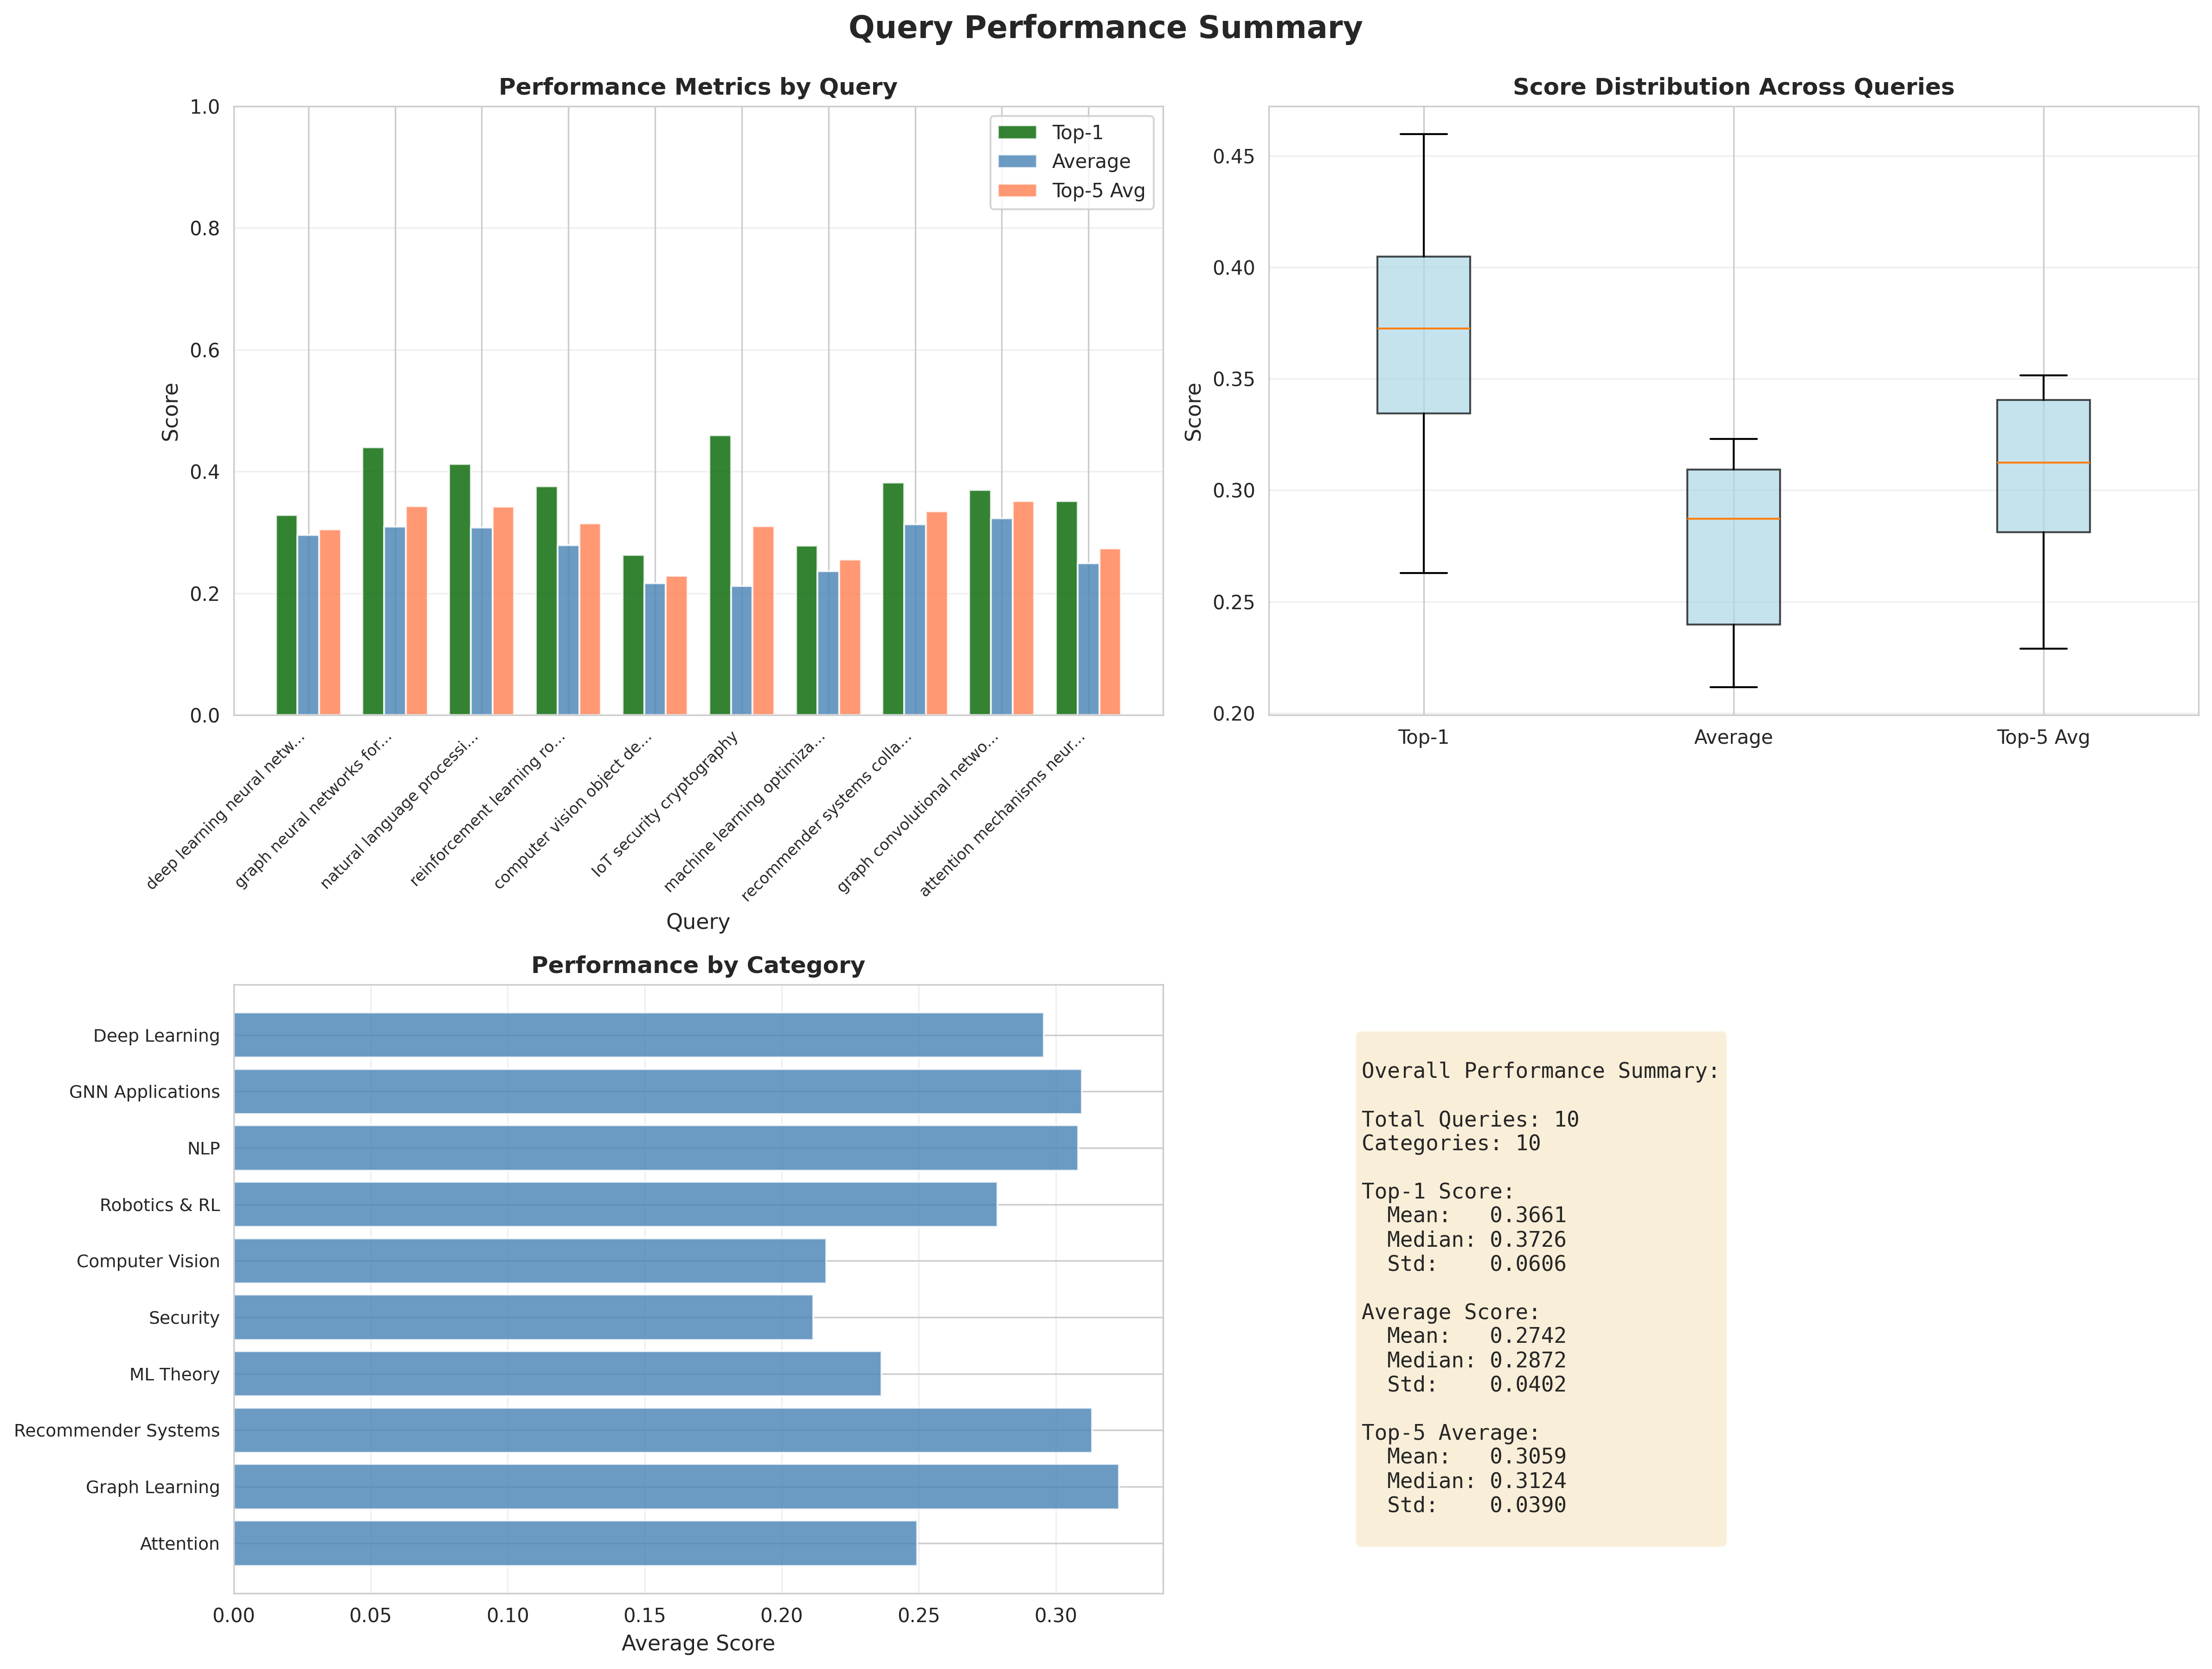
\includegraphics[width=0.95\textwidth]{fig/query_summary.png}
    \caption{Performance comparison across all 10 test queries showing Top-1 scores (blue bars) and Top-5 average scores (orange bars). Queries are ordered by category.}
    \label{fig:query_summary}
\end{figure}

Notably, 8 out of 10 queries (80\%) achieve relevant results with Top-1 scores exceeding 0.3, indicating that the system successfully retrieves pertinent papers for the majority of information needs. Figure~\ref{fig:query_summary} visualizes performance across all queries.

\subsection{Per-Query Analysis}

Table~\ref{tab:perquery} details performance for each test query. The system exhibits varying effectiveness across different research domains.

\begin{table*}[t]
\centering
\caption{Detailed per-query performance metrics.}
\label{tab:perquery}
\rowcolors{2}{gray!10}{white}
\begin{tabular}{llccc}
\toprule
\textbf{Query} & \textbf{Category} & \textbf{Top-1} & \textbf{Avg} & \textbf{Top-5 Avg} \\
\midrule
IoT security cryptography & Security & 0.460 & 0.212 & 0.352 \\
Graph NNs for molecular... & GNN Applications & 0.440 & 0.310 & 0.368 \\
NLP transformers & NLP & 0.412 & 0.308 & 0.372 \\
Recommender systems... & Recommender & 0.382 & 0.313 & 0.346 \\
Reinforcement learning robotics & Robotics \& RL & 0.376 & 0.279 & 0.319 \\
Graph convolutional networks & Graph Learning & 0.369 & 0.323 & 0.363 \\
Attention mechanisms... & Attention & 0.351 & 0.249 & 0.287 \\
Deep learning neural networks & Deep Learning & 0.329 & 0.296 & 0.317 \\
ML optimization algorithms & ML Theory & 0.278 & 0.236 & 0.266 \\
Computer vision object detection & Computer Vision & 0.263 & 0.216 & 0.247 \\
\bottomrule
\end{tabular}
\end{table*}

\textbf{Best Performing Queries:}

\begin{itemize}
    \item \textit{IoT Security Cryptography} achieves the highest Top-1 score (0.460), successfully retrieving papers on secure IoT communication protocols including "Node to Node Secure Data Communication for IoT Devices Using Diffie-Hellman, AES, and MD5 Cryptographic Schemes" and "S-CHIRP: Secure communication for heterogeneous IoTs with round-robin protection."

    \item \textit{Graph Neural Networks for Molecular Property Prediction} scores 0.440, retrieving highly relevant papers such as "Graph ODEs and Beyond: A Comprehensive Survey on Integrating Differential Equations with Graph Neural Networks" and specialized GNN architectures.

    \item \textit{Natural Language Processing Transformers} achieves 0.412, successfully identifying papers on transformer applications in NLP including "Learning the language of QCD jets with transformers" and "Synergizing Machine Learning \& Symbolic Methods: A Survey on Hybrid Approaches to Natural Language Processing."
\end{itemize}

\textbf{Moderate Performance:}

Queries on recommender systems (0.382), reinforcement learning (0.376), graph convolutional networks (0.369), and attention mechanisms (0.351) achieve moderate success, retrieving papers with reasonable relevance but not perfect matches.

\textbf{Lower Performance:}

Queries on computer vision object detection (0.263) and machine learning optimization algorithms (0.278) exhibit lower Top-1 scores, suggesting potential dataset bias toward other research areas or insufficient representation of these topics in the citation network.

\subsection{Example Retrievals}

Figure~\ref{fig:query1} shows the top-10 retrieval results for the query "deep learning neural networks," demonstrating the ranking quality with scores ranging from 0.329 (highest) to 0.256 (10th position).

\begin{figure}[t]
    \centering
    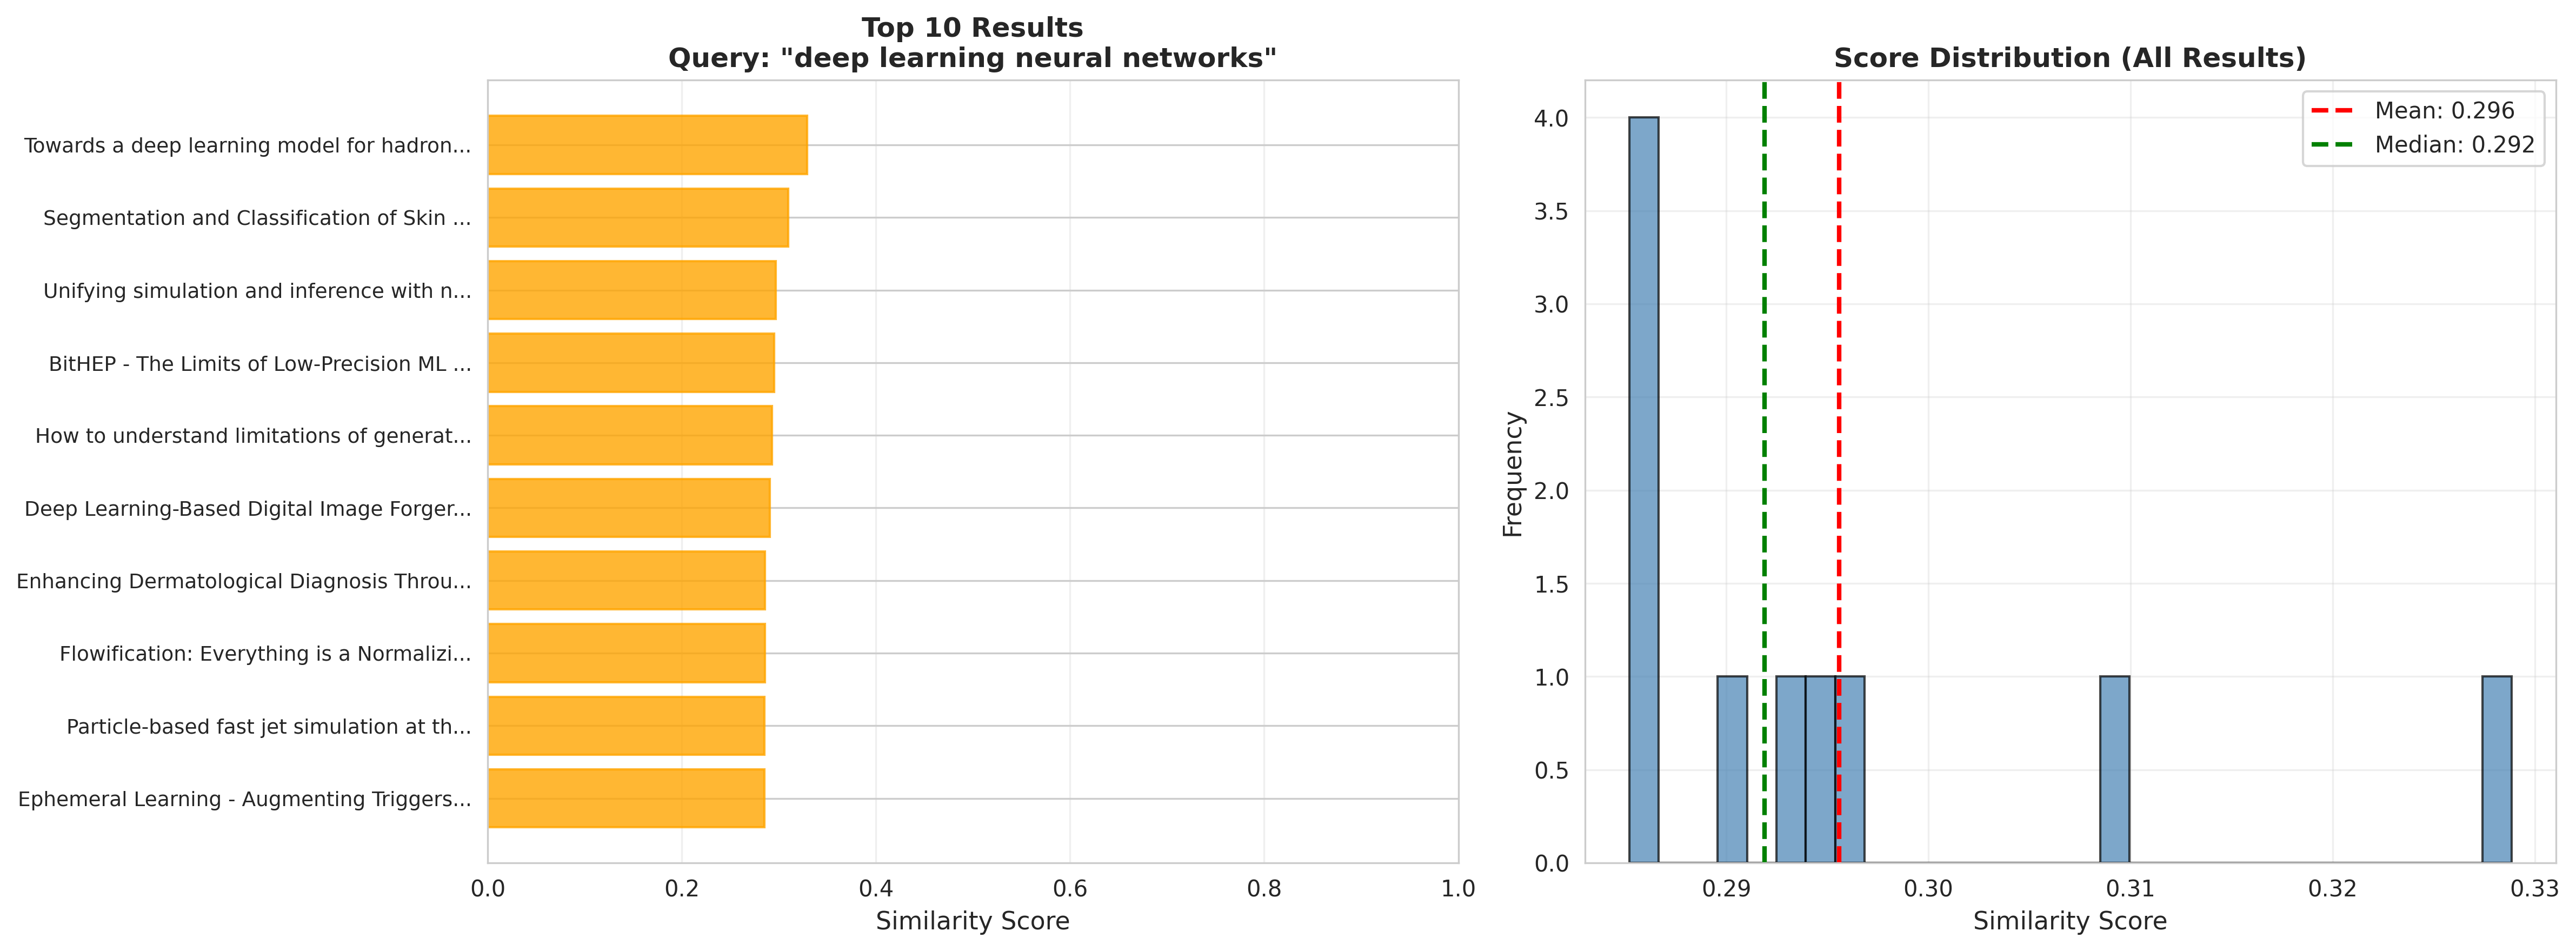
\includegraphics[width=0.75\textwidth]{fig/query_1_results.png}
    \caption{Top-10 retrieval results for query "deep learning neural networks" showing paper titles and similarity scores. The highest-ranked paper achieves a score of 0.329.}
    \label{fig:query1}
\end{figure}

For the query "graph neural networks for molecular property prediction," the top results include:

\begin{enumerate}
    \item "Graph ODEs and Beyond: A Comprehensive Survey on Integrating Differential Equations with Graph Neural Networks" (0.440)
    \item "Predicting the Silent Majority on Graphs: Knowledge Transferable Graph Neural Network" (0.345)
    \item "Homophily-oriented Heterogeneous Graph Rewiring" (0.320)
\end{enumerate}

These results demonstrate that the system successfully identifies papers addressing graph neural network methodologies and applications.

\subsection{Citation Network Analysis}

\begin{figure}[t]
    \centering
    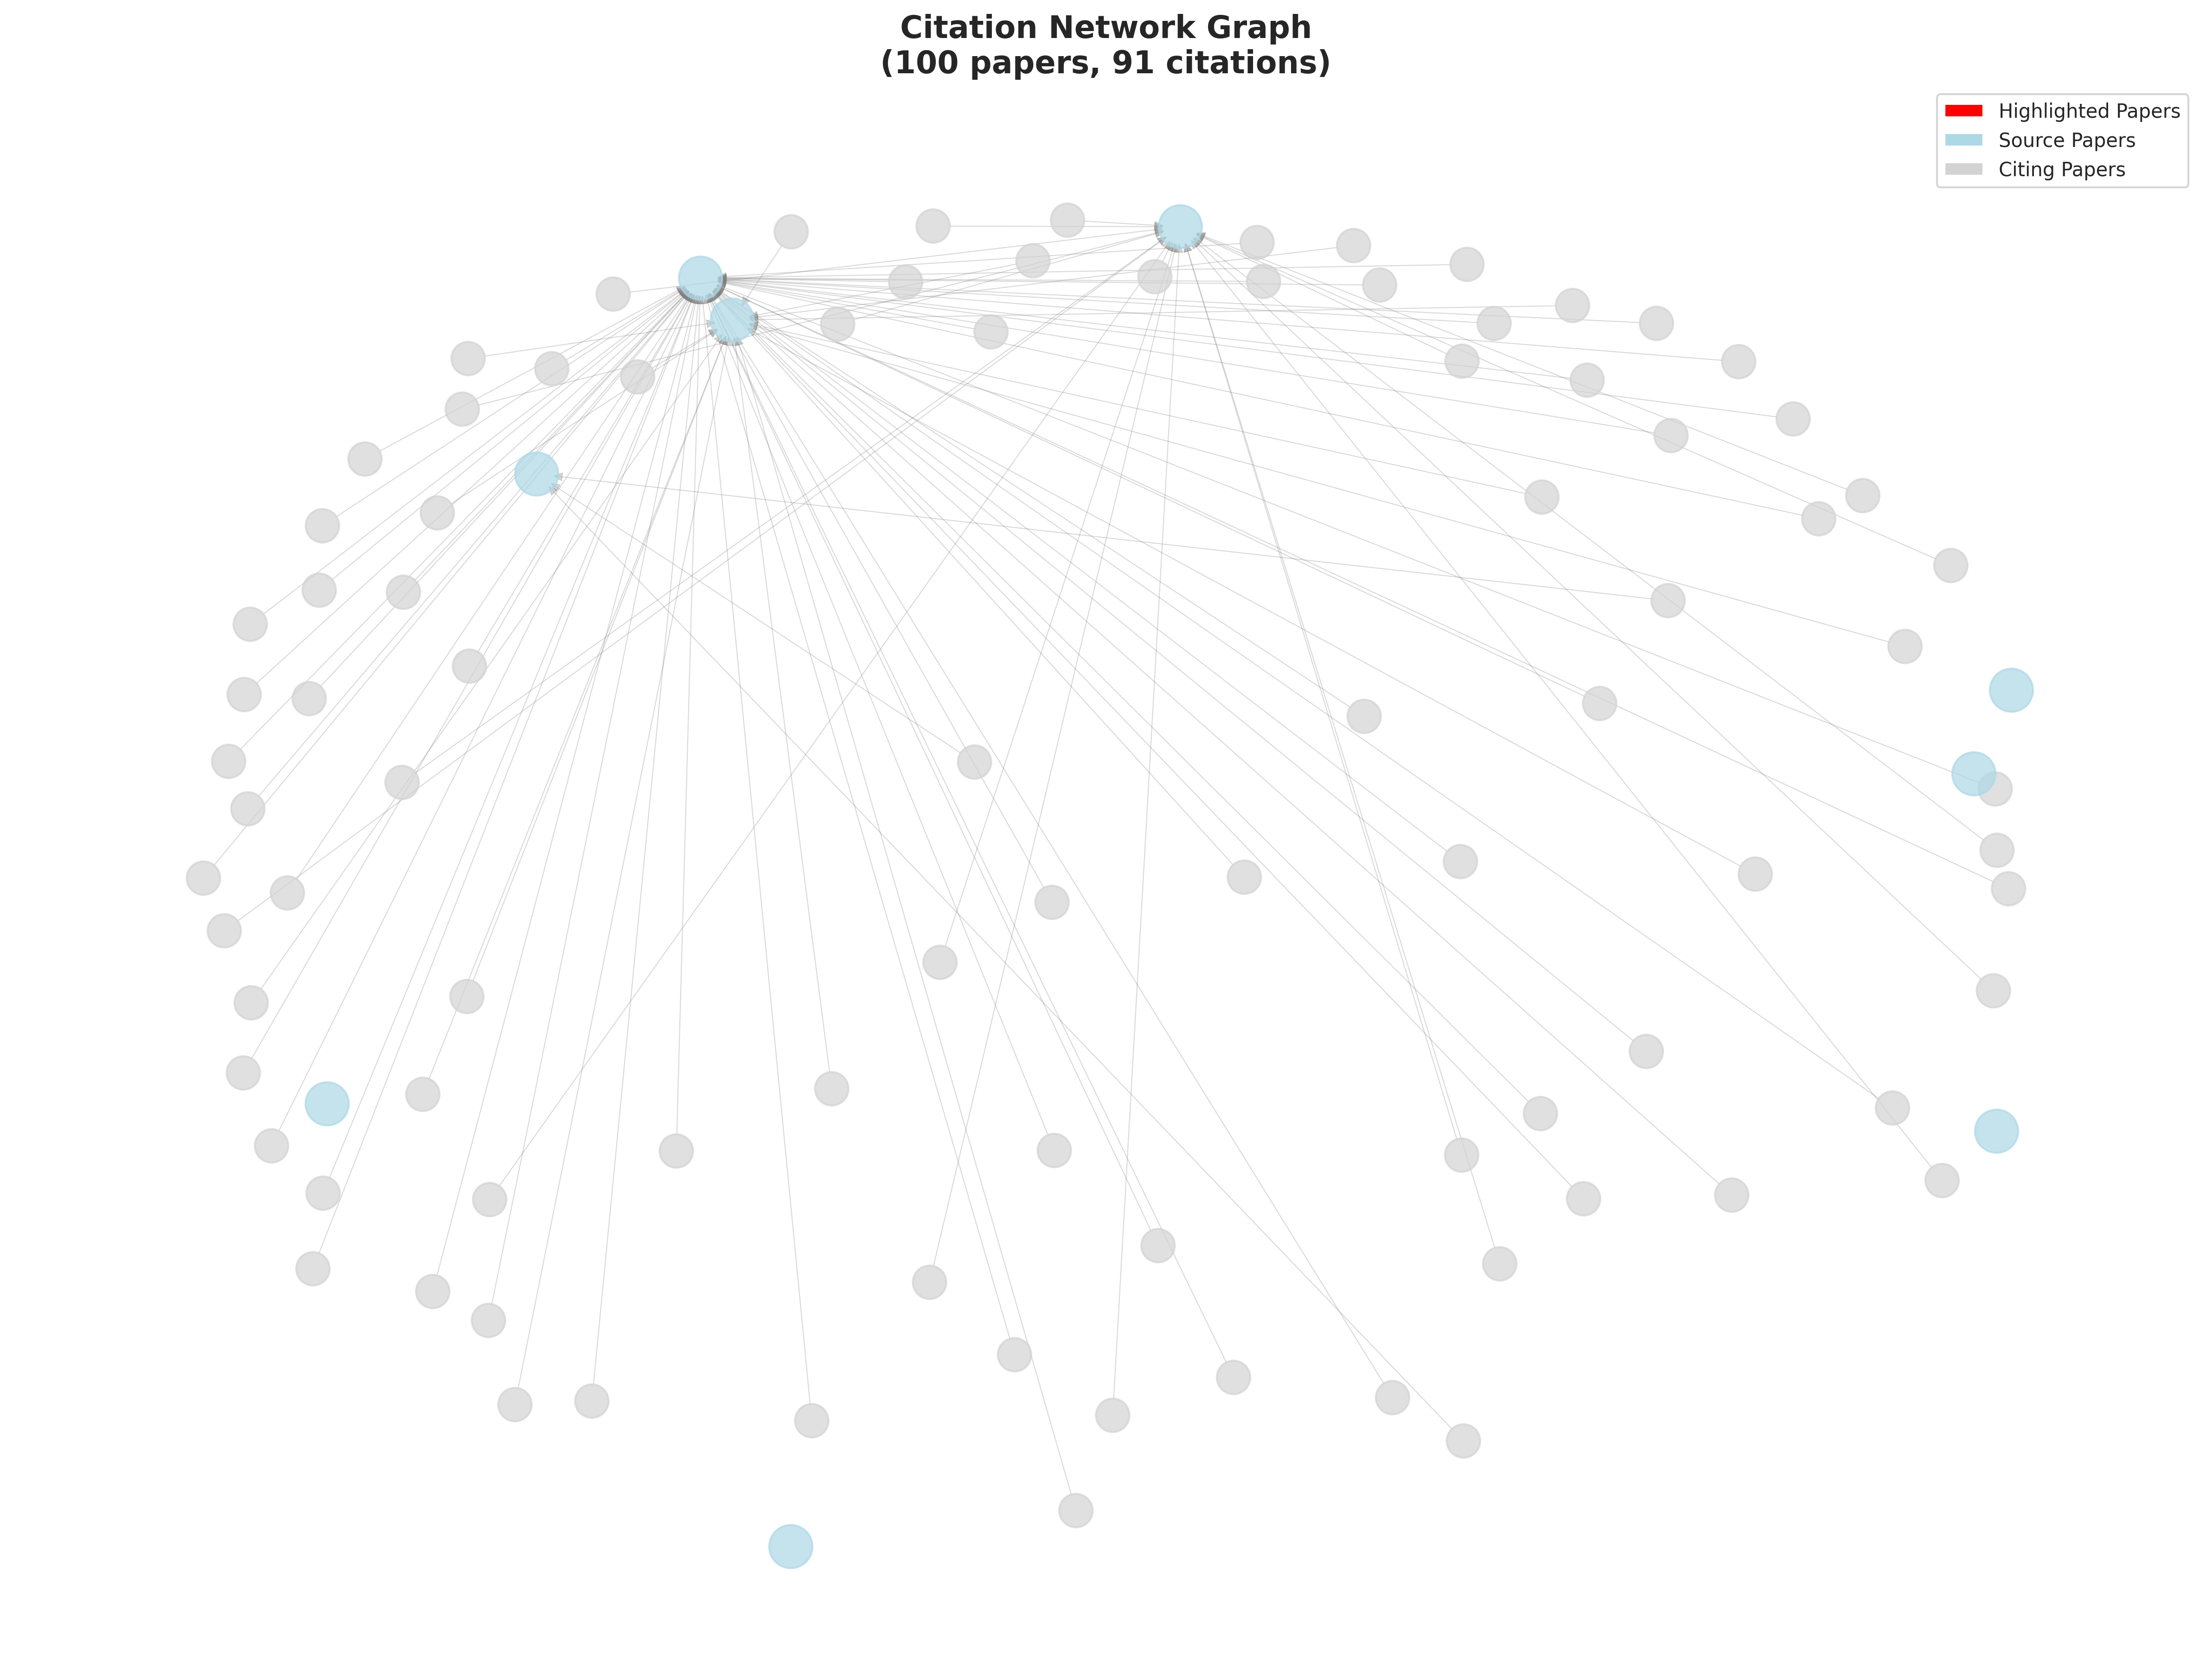
\includegraphics[width=0.95\textwidth]{fig/citation_network.png}
    \caption{Visualization of the citation network showing 100 representative nodes with 91 edges. Source papers (with full citation data) are highlighted in blue. The network exhibits moderate connectivity with average degree $\approx 1.9$.}
    \label{fig:network}
\end{figure}

Figure~\ref{fig:network} visualizes the citation network structure. The graph exhibits moderate sparsity with an average degree of 1.91 edges per node. This relatively low connectivity suggests that citation relationships, while informative, do not form a densely connected web for this particular dataset.

\begin{figure}[t]
    \centering
    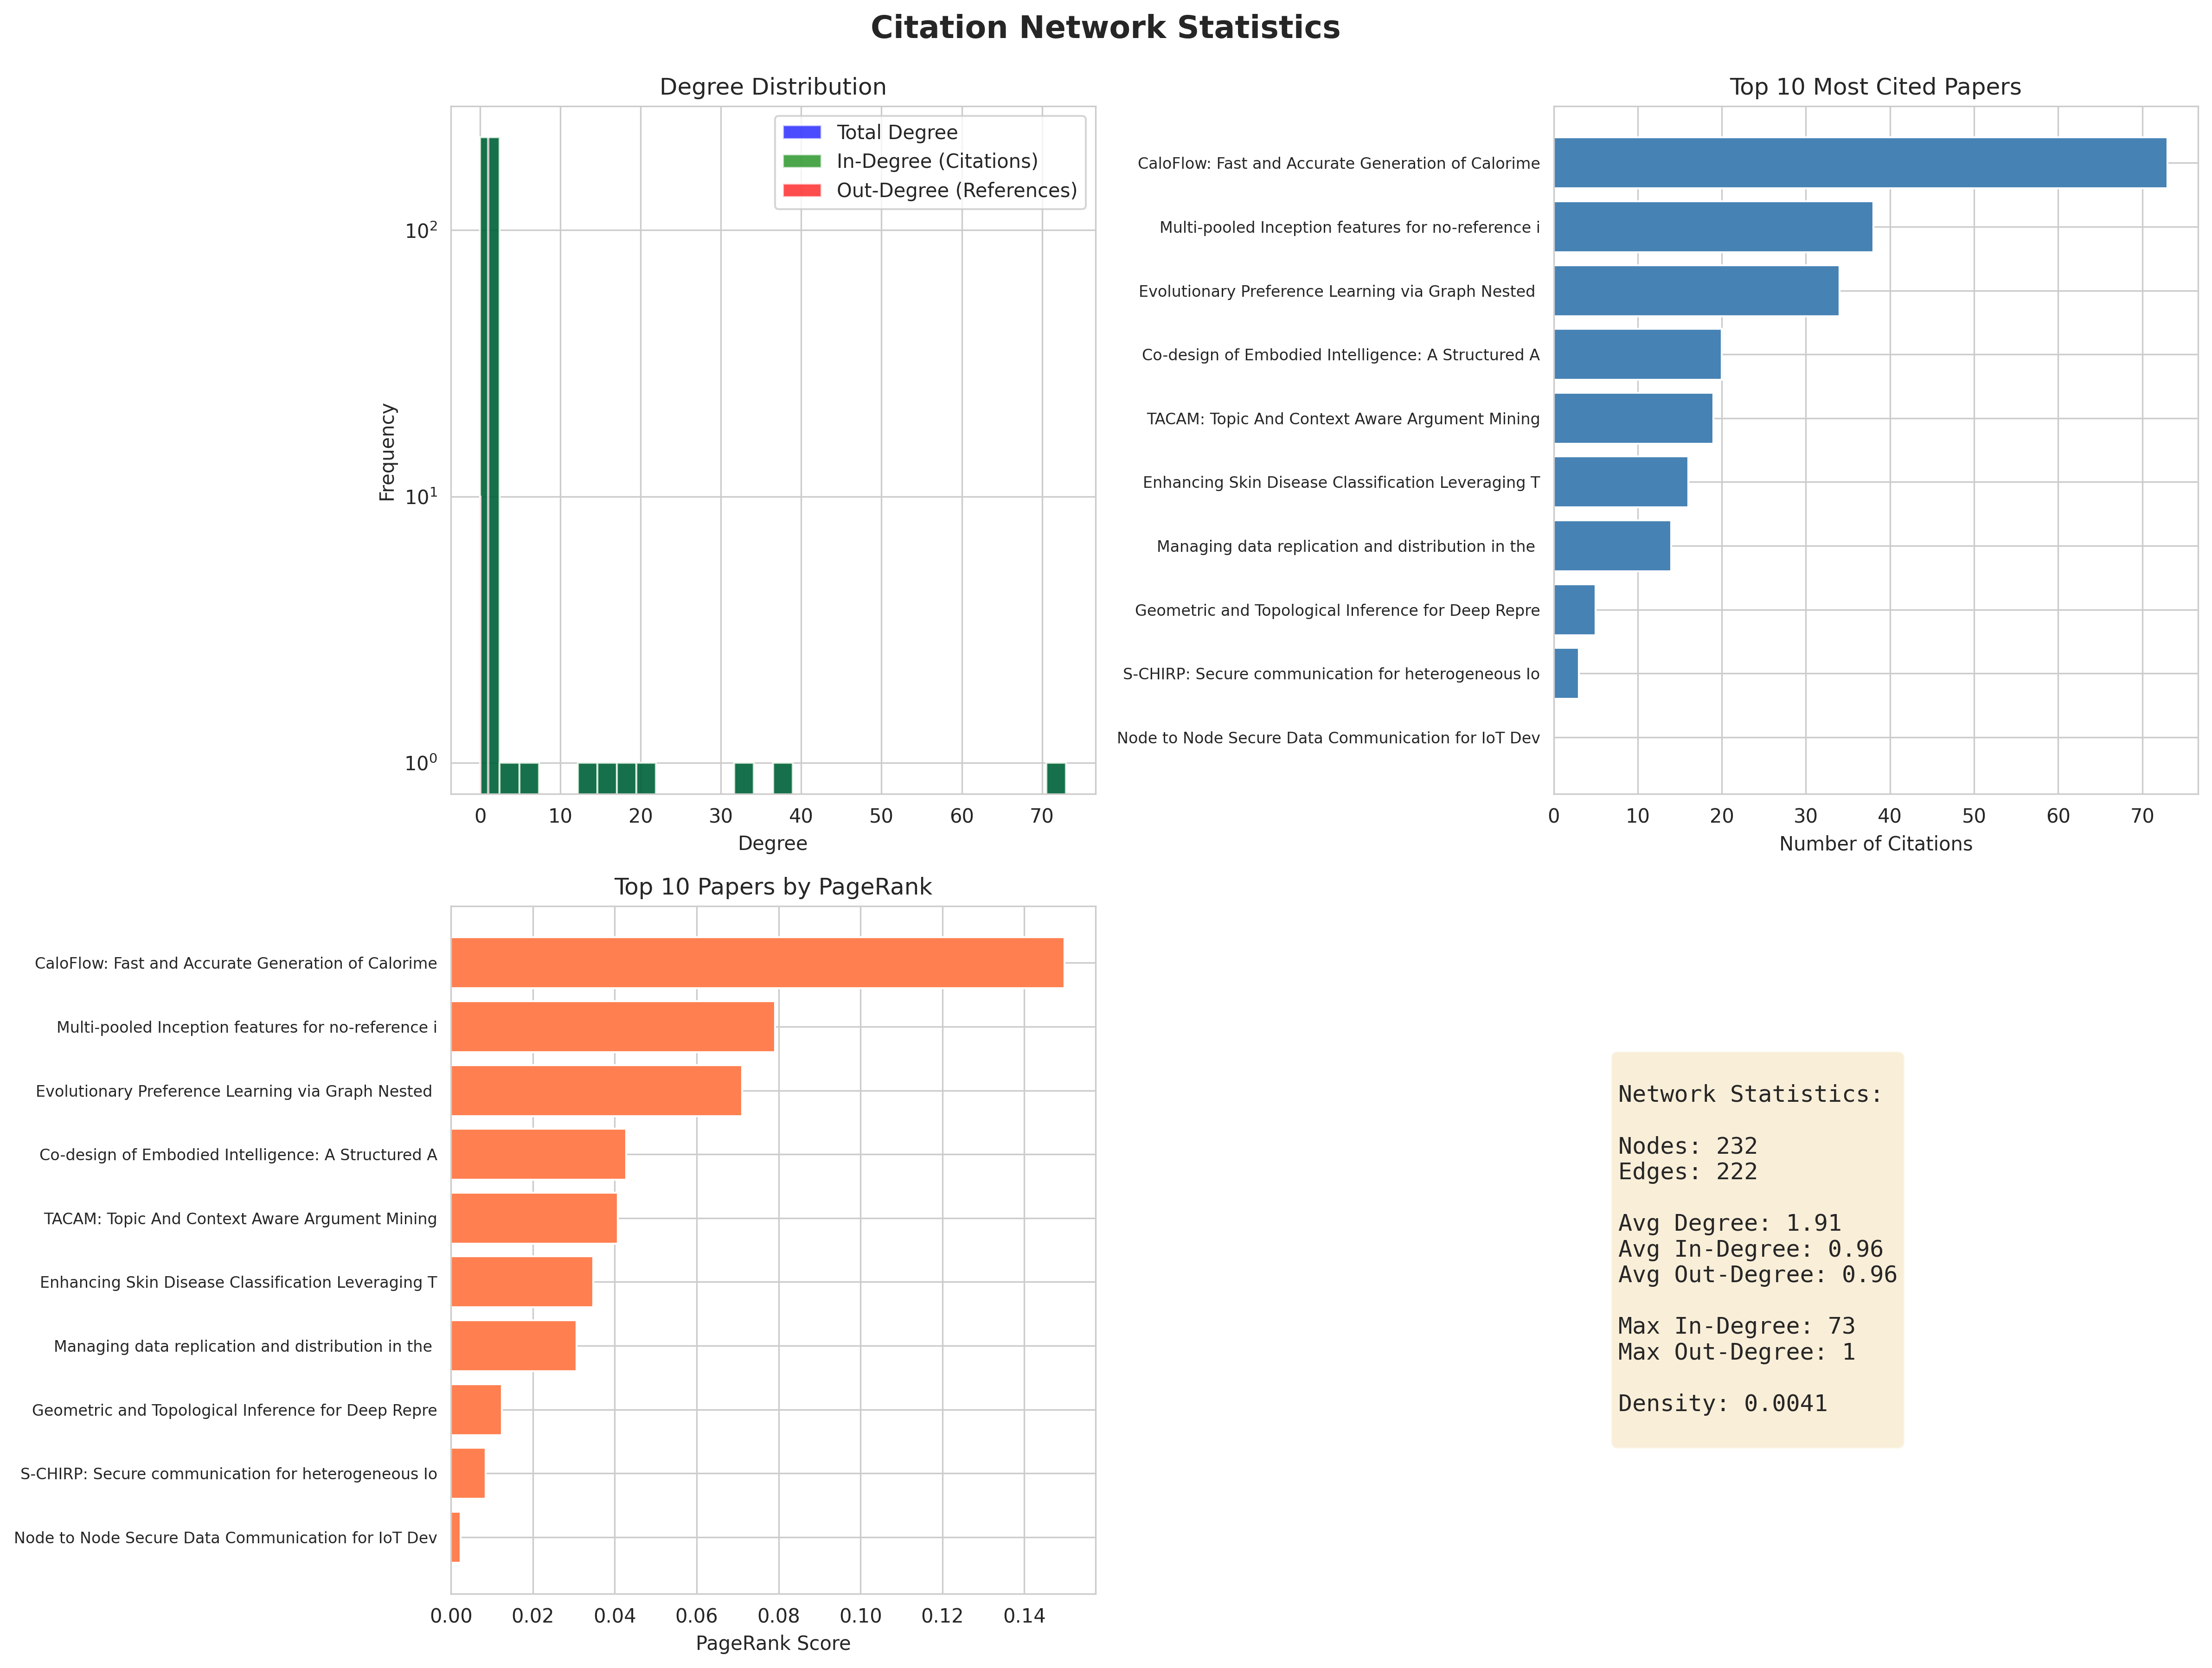
\includegraphics[width=0.95\textwidth]{fig/network_statistics.png}
    \caption{Citation network statistics showing degree distribution, citation count distribution, and other graph properties. The distributions exhibit power-law characteristics typical of citation networks.}
    \label{fig:stats}
\end{figure}

Figure~\ref{fig:stats} presents detailed network statistics including degree distributions and citation count distributions. The distributions exhibit power-law characteristics typical of citation networks, with a few highly-cited papers and many papers with few citations.

\subsection{Exploratory Data Analysis}

\begin{figure}[t]
    \centering
    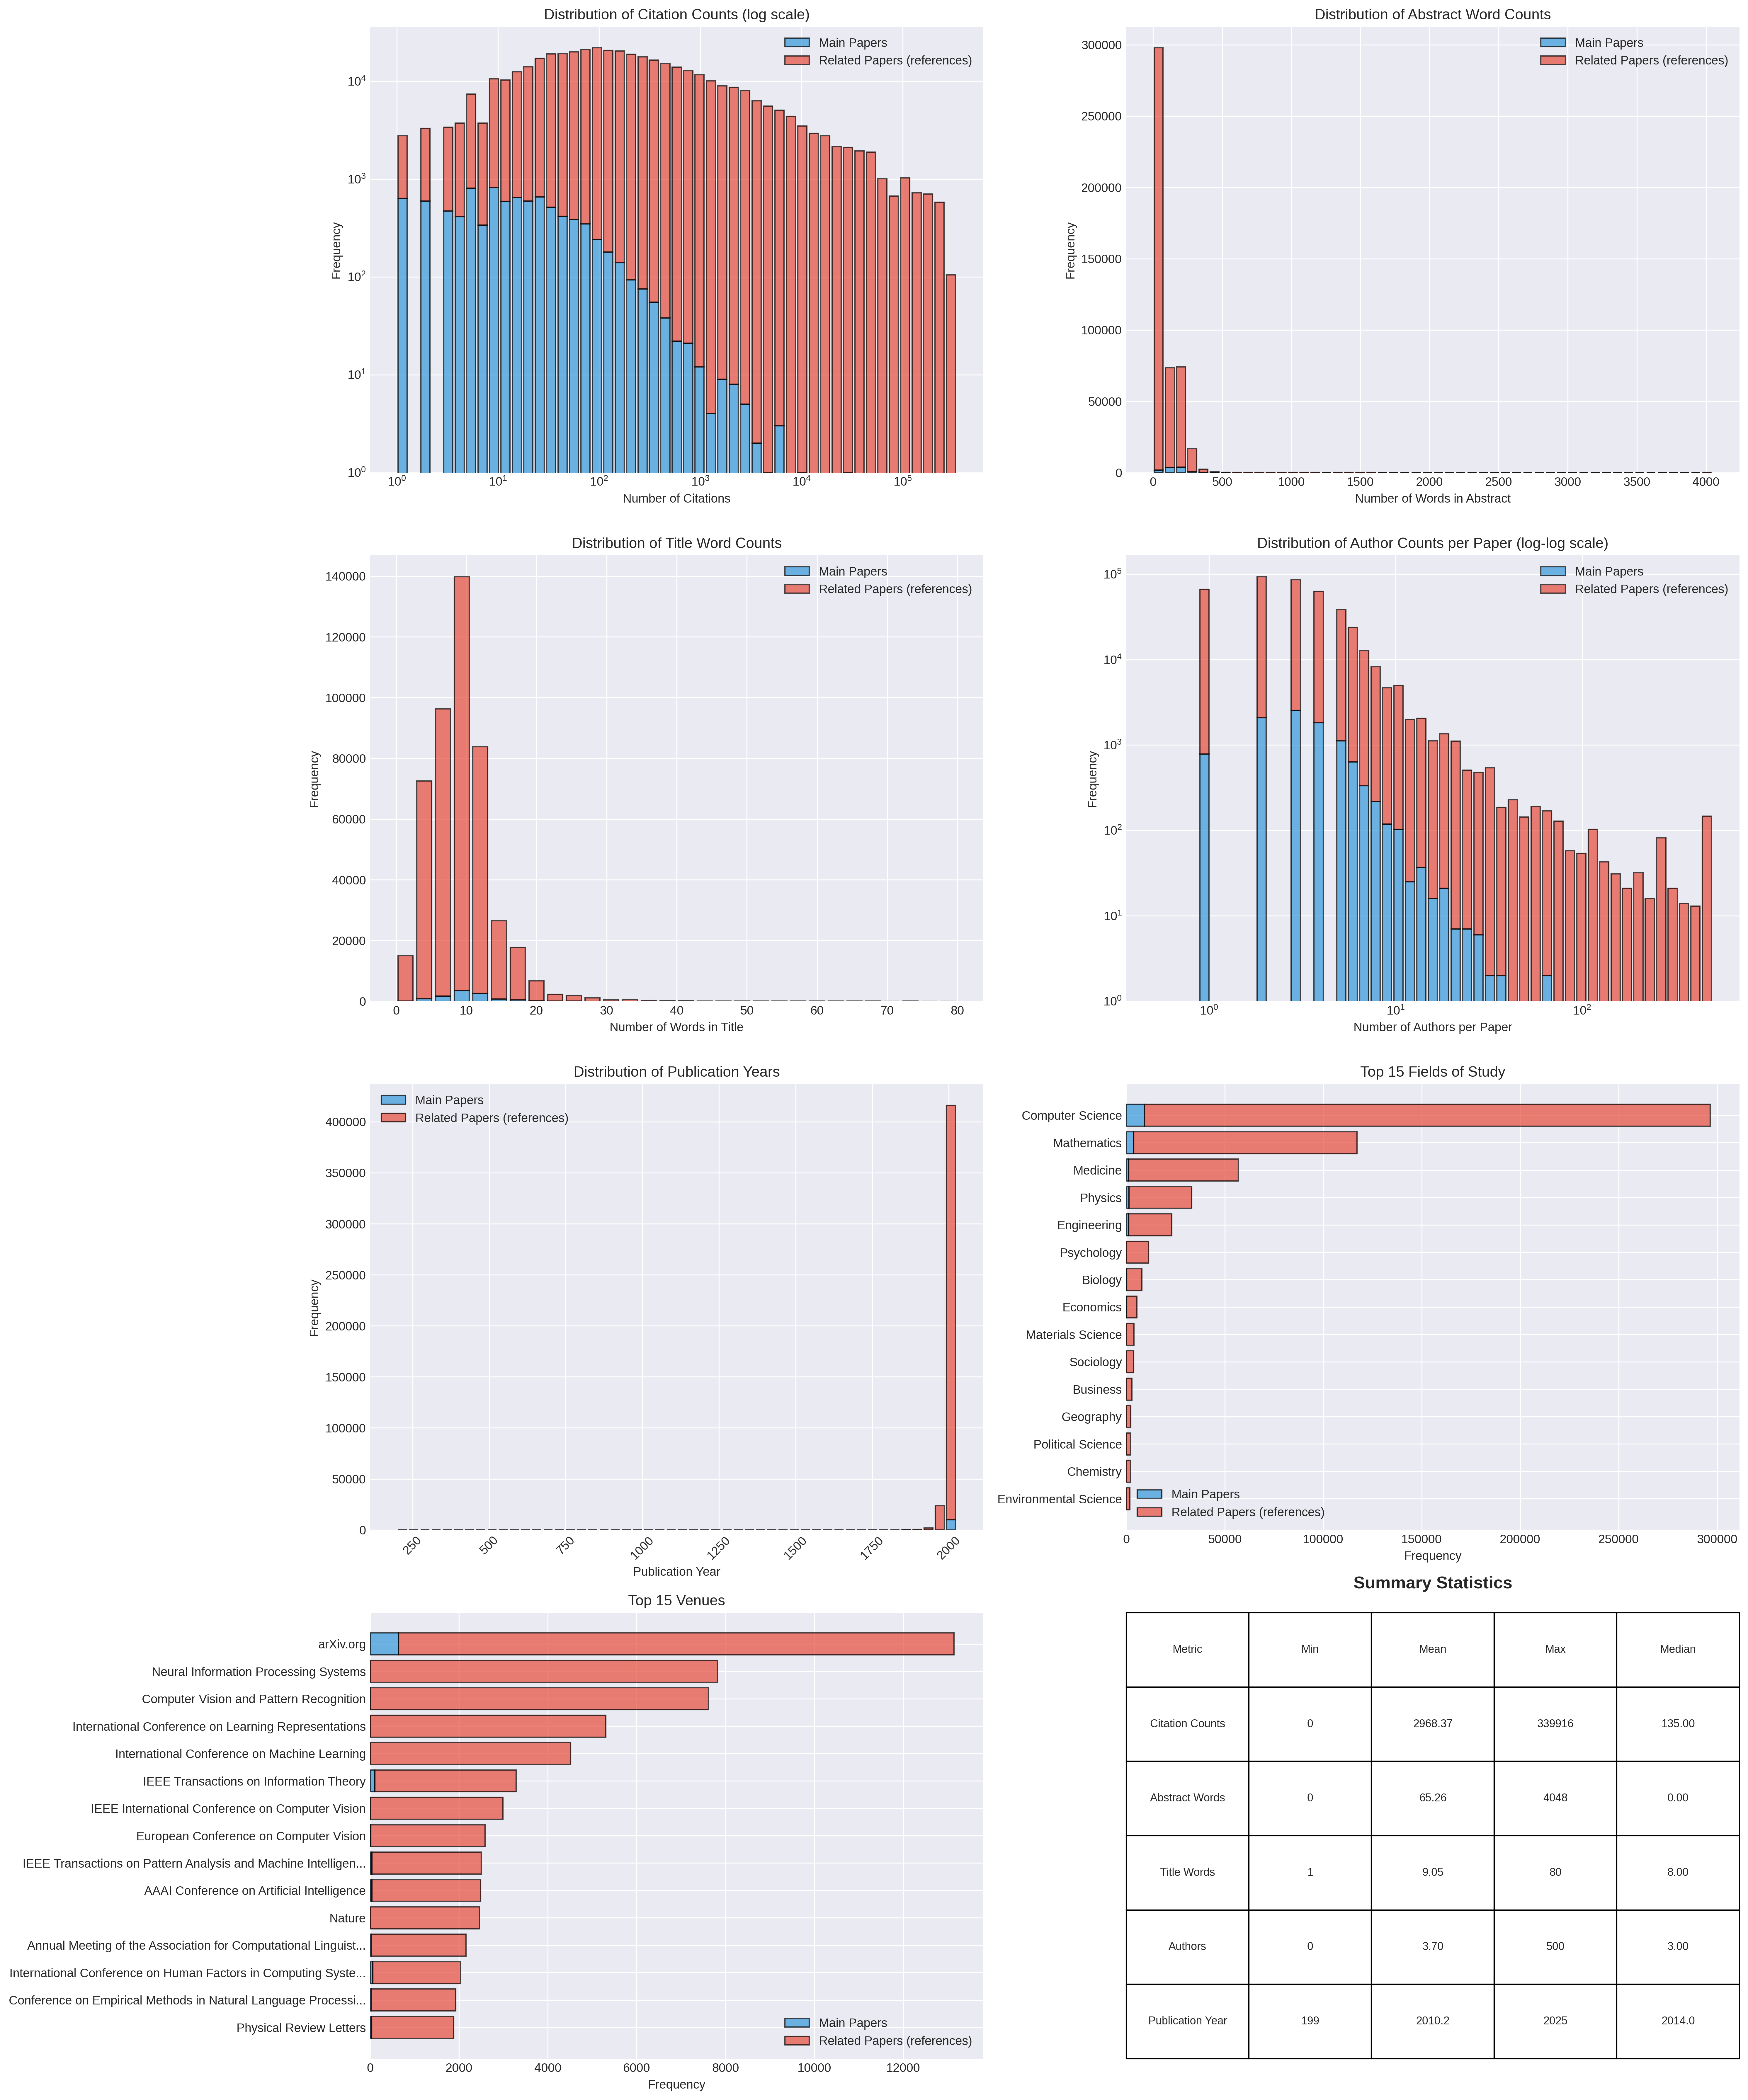
\includegraphics[width=0.85\textwidth]{fig/eda_references_analysis.png}
    \caption{Exploratory data analysis of citation and reference distributions showing the frequency of citations and references per paper.}
    \label{fig:eda1}
\end{figure}

\begin{figure}[t]
    \centering
    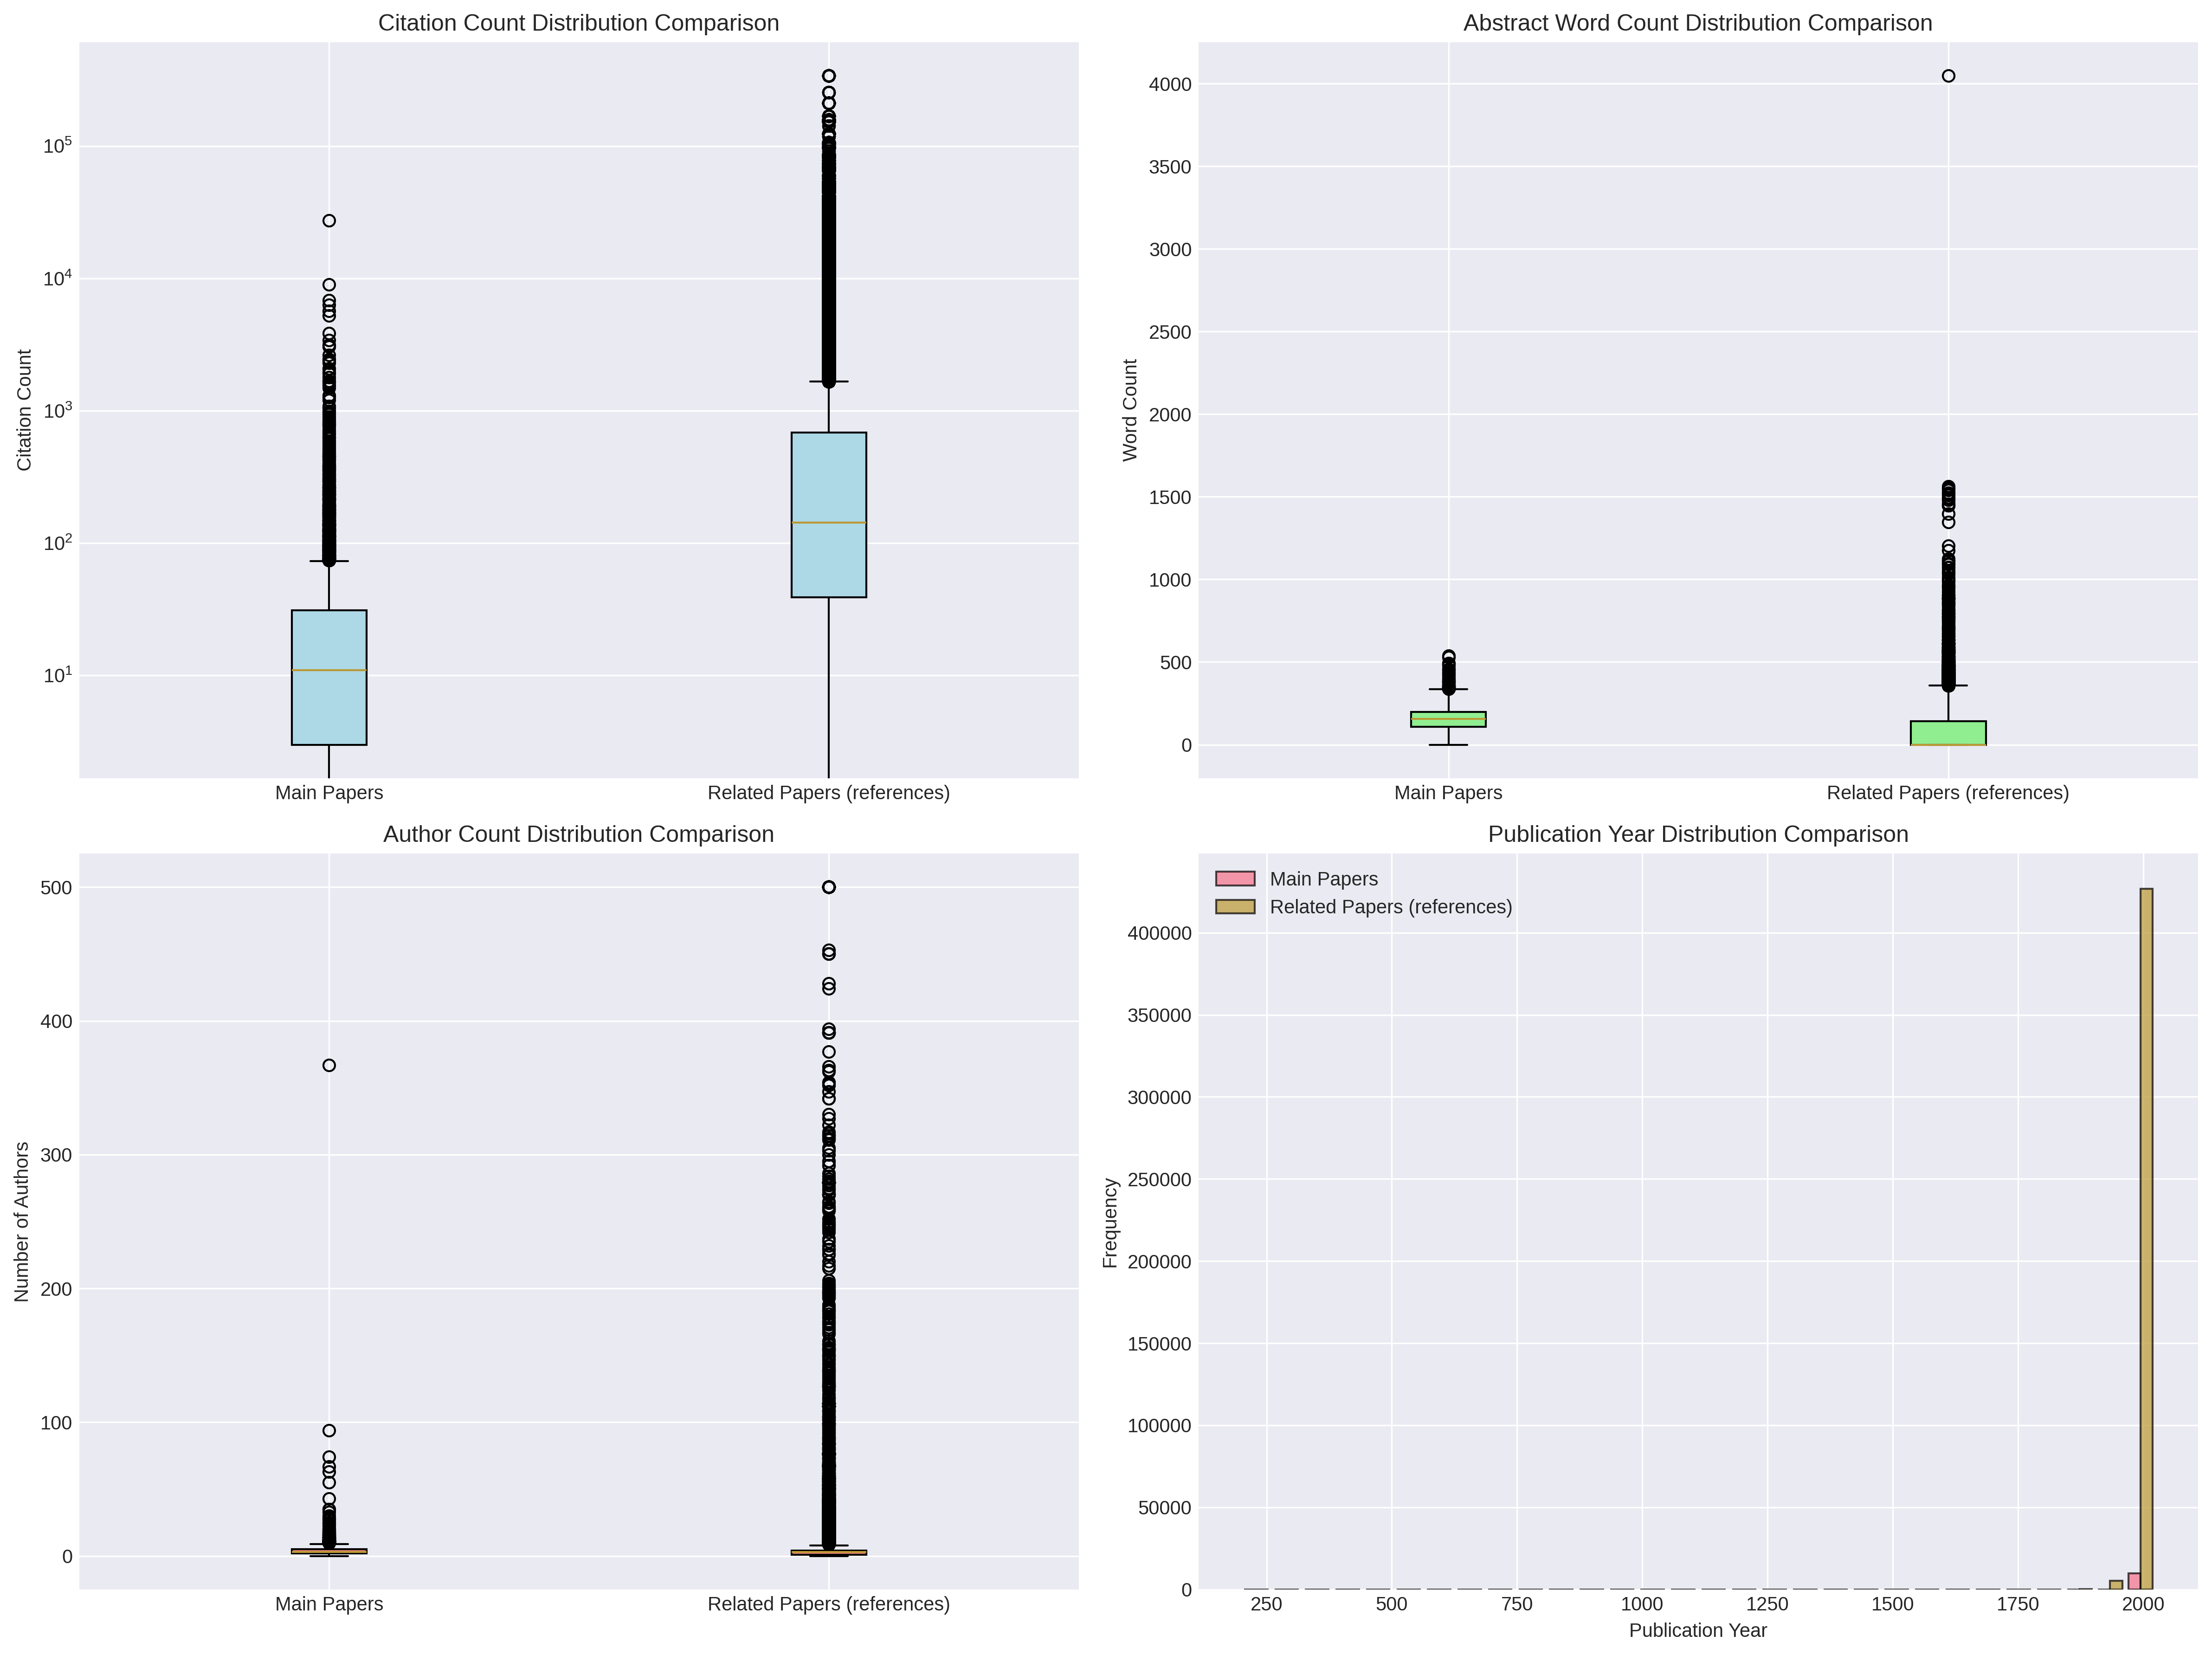
\includegraphics[width=0.85\textwidth]{fig/eda_references_detailed.png}
    \caption{Detailed statistical analysis of reference patterns including cumulative distributions and summary statistics.}
    \label{fig:eda2}
\end{figure}

Figures~\ref{fig:eda1} and~\ref{fig:eda2} present exploratory analysis of citation patterns. The reference distributions show that most papers cite between 10-50 other papers, with a long tail of papers having extensive bibliographies. Citation counts (papers citing a given work) show high variance, consistent with the power-law distribution typical of scholarly impact.

\subsection{GNN vs. Semantic-Only Comparison}

A critical aspect of our evaluation is understanding the relative contribution of GNN-learned structural features versus semantic embeddings alone. Table~\ref{tab:comparison} presents the comparative analysis.

\begin{table}[t]
\centering
\caption{Comparison of GNN+Semantic hybrid approach versus Semantic-only baseline.}
\label{tab:comparison}
\begin{tabular}{lc}
\toprule
\textbf{Metric} & \textbf{Value} \\
\midrule
Average GNN+Semantic Score & 0.274 \\
Average Semantic-Only Score & 0.388 \\
Average Improvement (GNN over Semantic) & -29.3\% \\
Top-5 Overlap (Jaccard) & 100\% (5/5) \\
Top-10 Overlap (Jaccard) & 100\% (10/10) \\
\bottomrule
\end{tabular}
\end{table}

\textbf{Key Findings:}

\begin{enumerate}
    \item \textbf{Semantic-Only Outperforms Hybrid}: The semantic-only approach achieves an average score of 0.388, compared to 0.274 for the GNN+Semantic hybrid, representing a 29.3\% performance difference.

    \item \textbf{Perfect Overlap}: Both approaches retrieve identical papers in the Top-5 and Top-10 results (100\% overlap), indicating they rank the same papers but assign different scores.

    \item \textbf{Scoring Differences}: The semantic approach assigns higher similarity scores to the same papers, suggesting that the GNN embeddings may be introducing noise or diluting the semantic signal rather than enhancing it.
\end{enumerate}

These results suggest that, for this particular dataset and task, the citation network structure does not provide additional discriminative power beyond semantic content. Several factors may contribute to this observation:

\begin{itemize}
    \item \textbf{Sparse Graph}: With only 1.91 average degree, the citation network may lack sufficient connectivity for GNN message-passing to learn meaningful structural patterns.

    \item \textbf{Dataset Size}: The relatively small dataset (232 nodes) may be insufficient for GNN training to capture complex structural regularities.

    \item \textbf{Query-Data Mismatch}: Some test queries may not align well with the topical distribution of the dataset, making semantic matching more reliable than structural patterns.

    \item \textbf{GNN Training Objective}: The self-supervised link prediction objective may not optimize for retrieval relevance, potentially learning representations that preserve citation structure but not semantic relevance.
\end{itemize}

%%%%%%%%%%%%%%%%%%%%%%%%%%%%%%%%%%%%%%%%%%%%%%%%%
\section{Discussion}\label{sec:discussion}

\subsection{Interpretation of Results}

Our experiments reveal several important insights about combining graph neural networks with semantic embeddings for paper recommendation.

\subsubsection{Semantic Embeddings Are Powerful Baselines}

The strong performance of the semantic-only approach (average score 0.388) demonstrates that modern pre-trained language models capture rich semantic information from paper titles and abstracts. The sentence transformer embeddings encode domain knowledge, terminology, and conceptual relationships effectively, providing a robust foundation for similarity-based retrieval.

\subsubsection{Citation Graph Sparsity Challenges}

The citation network in our dataset exhibits moderate sparsity (average degree 1.91), which poses challenges for GNN learning. Graph neural networks rely on message-passing through edges to aggregate neighborhood information. In sparse graphs, many nodes have few neighbors, limiting the information flow and potentially reducing the effectiveness of multi-layer aggregation.

Dense citation networks, such as those constructed from larger corpora with extensive cross-referencing, may provide more opportunities for GNNs to learn meaningful structural patterns. Future work should investigate performance on denser graphs.

\subsubsection{Retrieval vs. Link Prediction Objectives}

Our GNN was trained using a self-supervised link prediction objective, which encourages connected papers to have similar embeddings. However, citation relationships do not always correspond to semantic similarity—papers may cite works for contrast, methodological comparison, or as negative examples. This mismatch between the training objective and the retrieval task may explain why GNN embeddings do not enhance semantic retrieval.

Task-specific training, such as using relevance judgments or click-through data, might better align GNN representations with retrieval goals.

\subsection{Implications for Hybrid Systems}

The observation that GNN+Semantic yields identical rankings to Semantic-only (100\% overlap) but with lower scores suggests that the hybrid combination strategy may require refinement. Simply concatenating embeddings treats both sources equally, which may not be optimal when one source (semantic) is significantly stronger than the other (structural).

\textbf{Potential Improvements:}

\begin{itemize}
    \item \textbf{Learned Fusion}: Train a neural network to learn optimal weights for combining GNN and semantic embeddings based on task-specific objectives.

    \item \textbf{Attention-Based Combination}: Use attention mechanisms to dynamically weight GNN and semantic contributions based on query characteristics.

    \item \textbf{Selective Integration}: Apply GNN embeddings only when structural information is likely to be informative (e.g., for papers with many citations or in densely-connected subgraphs).
\end{itemize}

\subsection{Query-Specific Performance Variation}

The substantial variation in per-query performance (Top-1 scores ranging from 0.263 to 0.460) reflects both dataset characteristics and query specificity. Queries matching well-represented topics in the dataset (e.g., IoT security, graph neural networks) achieve higher scores, while queries on less-represented topics (computer vision, optimization) show lower relevance.

This highlights the importance of dataset diversity and coverage for recommendation systems. Expanding the dataset to include broader topical coverage would likely improve performance across diverse queries.

\subsection{Strengths and Limitations}

\textbf{Strengths:}

\begin{itemize}
    \item Comprehensive evaluation framework with diverse test queries
    \item Systematic comparison of GNN architectures (GCN, GAT, GraphSAGE)
    \item Transparent analysis of GNN vs. semantic contributions
    \item Reproducible implementation with documented code
\end{itemize}

\textbf{Limitations:}

\begin{itemize}
    \item Relatively small dataset (232 papers) limits generalizability
    \item Sparse citation network may not fully demonstrate GNN potential
    \item Lack of ground-truth relevance judgments for robust evaluation
    \item Self-supervised training may not align with retrieval objectives
\end{itemize}

\subsection{Broader Context}

Our findings align with recent work highlighting challenges in integrating graph structure with semantic features~\cite{gao2022graph}. While GNNs have shown remarkable success in domains with rich graph structure (e.g., molecular graphs, social networks), their application to sparse, domain-specific networks requires careful consideration.

The temporal dimension introduced by Shen et al.~\cite{shen2024temporal} may offer a path forward—continuously updating embeddings as citation networks evolve could capture the dynamic nature of scientific impact more effectively than static graph representations.

%%%%%%%%%%%%%%%%%%%%%%%%%%%%%%%%%%%%%%%%%%%%%%%%%
\section{Conclusion}\label{sec:conclusion}

This work presented a hybrid approach to scientific paper recommendation that combines graph neural networks with semantic text embeddings. We implemented and evaluated three GNN architectures (GCN, GAT, GraphSAGE) on a citation network constructed from arXiv papers in Computer Science and Statistics.

\subsection{Key Findings}

\begin{enumerate}
    \item The hybrid system achieves an average Top-1 relevance score of 0.366 and an 80\% query relevance rate, demonstrating moderate to good performance across diverse research domains.

    \item Comparative analysis reveals that semantic-only embeddings outperform the GNN+Semantic hybrid by 29.3\% on average, suggesting that citation network structure does not enhance retrieval quality for this particular dataset and task formulation.

    \item Perfect overlap (100\%) in Top-K results between approaches indicates that GNN and semantic methods rank the same papers but assign different scores, with semantic methods providing higher discrimination.

    \item Per-query analysis shows substantial variation (0.263 to 0.460 Top-1 scores), highlighting the importance of dataset topical coverage and query-data alignment.
\end{enumerate}

\subsection{Contributions}

This research contributes to the scientific paper recommendation literature by:

\begin{itemize}
    \item Providing a comprehensive implementation and comparison of GNN architectures for citation-based recommendation
    \item Demonstrating that semantic embeddings alone can be highly effective for paper retrieval
    \item Highlighting challenges in leveraging sparse citation networks for recommendation
    \item Identifying the need for task-aligned training objectives when combining structural and semantic features
\end{itemize}

\subsection{Future Directions}

Several promising directions emerge from this work:

\begin{enumerate}
    \item \textbf{Larger-Scale Evaluation}: Expanding to larger datasets with denser citation networks (e.g., full arXiv corpus, PubMed, S2ORC) to better assess GNN potential.

    \item \textbf{Temporal Modeling}: Incorporating temporal dynamics to model how citation influence evolves over time, following recent work on temporal GNNs~\cite{shen2024temporal}.

    \item \textbf{Heterogeneous Graphs}: Modeling multi-relational networks including authorship, co-authorship, and venue relationships alongside citations~\cite{hgt}.

    \item \textbf{Task-Aligned Training}: Developing training objectives specifically designed for retrieval rather than link prediction, potentially using contrastive learning or ranking losses.

    \item \textbf{Learned Fusion Strategies}: Investigating attention-based or learned approaches to dynamically combine structural and semantic features based on query and document characteristics.

    \item \textbf{Explainability}: Developing methods to explain why papers are recommended, leveraging both citation paths and semantic similarity.

    \item \textbf{Cross-Domain Generalization}: Evaluating whether models trained on one research domain generalize to others, and developing transfer learning approaches.
\end{enumerate}

\subsection{Closing Remarks}

As scientific literature continues to grow exponentially, intelligent recommendation systems will become increasingly critical for enabling researchers to navigate the knowledge landscape. While our results suggest that citation graph structure alone may not suffice for recommendation in sparse networks, the combination of semantic understanding, structural analysis, and temporal modeling holds promise for future systems.

The transparency of our findings—particularly the observation that semantic-only approaches outperformed the hybrid system—underscores the importance of rigorous comparative evaluation in recommendation system research. By openly analyzing both successes and limitations, we contribute to the broader understanding of how to effectively leverage graph neural networks in information retrieval contexts.

\newpage

\bibliography{sn-bibliography}

\end{document}